\chapterimage{Week3Clarifier1.jpg} % Chapter heading image

\chapter{Liquid Treatment Part II}

\section{Secondary Treatment}\index{Secondary Treatment}
\begin{itemize}
\item While preliminary and primary treatment processes are designed primarily to remove solids from wastewater, secondary treatment is for the removal of organics.
\item Secondary treatment involves:
\begin{itemize}
\item biological conversion of the dissolved and suspended organics in wastewater into biomass, and
\item physical settling (separation) process where the solids including the biomass formed during secondary treatment is separated and removed from the treated wastewater.
\end{itemize}

\item With the removal of gross solids in the preliminary treatment followed by removable of settleable solids in the primary clarifiers and the removal of dissolved and suspended organics in the secondary treatment processes, the wastewater is considered treated.
\item Secondary treated wastewater is typically disposed or treated further for reuse or disposal (depending upon the end use/application and the NPDES permit stipulations).
\item The solids (biomass) removed from the secondary treatment is typically mixed with the solids from primary treatment and stabilized using a solids treatment process like sludge digestion prior to its disposal.
\end{itemize}
\vspace{1cm}

\textbf{Secondary treatment process incorporates one of the following three approaches:}


\subsection{Fixed film system}\index{Fixed Film System}	
		
Trickling filter is a fixed film secondary treatment process wherein the organic content of the wastewater is removed using biological growth attached to an inert media such as lava rock or plastic\\
\begin{center}
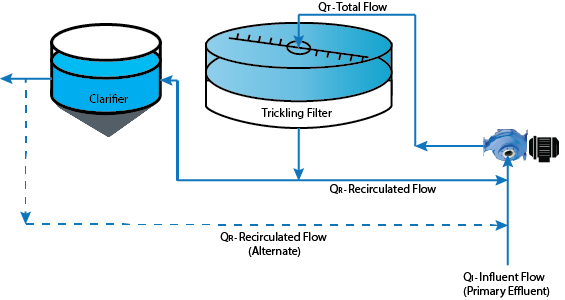
\includegraphics[scale=0.5]{TricklingFilter}
\end{center}		
\begin{itemize}
\item In a trickling filter, the wastewater is sprayed evenly on the surface of the media with a rotary type distributor with orifices
\item The wastewater percolates through the media bed, where it comes in contact with biological slime growth – zoogleal film (zooglea)
\item The aerobic biomass - bacteria, protozoa and other microoorganisms in the zooglea capture and consume the suspended and dissolved organics from the wastewater.
\item The microorganisms metabolize the organics and in the process produce more microbial mass resulting in increasing the thickness of the zoogleal layer.
\item The thickness of the zoogleal layer can only increase to a point until the wastewater flow – hydraulic load, shears the slime layer – “sloughs off” and is carried out as part of the effluent flow as sloughing.
\item The treated wastewater cascades from the bottom of the media into the underdrain system – lower portion of the TF comprised of columns which support the media base.  The underdrain has a sloping floor to direct the cascading water into a center channel .
\item The clarifier allows for the separation (settling) of the  of the solids (sloughed off material).  The settled solids is removed - typically pumped to a digester and the clarified effluent flows out of the clarifier.
\item The source of oxygen to support the aerobic growth is from the oxygen dissolved in the wastewater as it is sprayed over the media and from the air currents due to the downward flow of the wastewater and the temperature difference between ambient and the interior of the trickling filter.  Forced ventilation system may be designed as part of the trickling filter

\item Word trickling “filter” is a misnomer - no filtration is involved
\item Advantage includes process simplicity and lower costs
\item Disadvantage include BOD removal efficiency of only about 80-85%
\item The media may be rock, slag, coal, bricks, redwood blocks, molded plastic, or any other sound durable material.
\item The media depth ranges from about three to eight feet for rock media trickling filters and 15 to 30 feet for synthetic media.
\item The media needs to be uniformly sized and have adequate empty spaces (voids) to ensure maintaining aerobic condition necessary for the survival of biomass.  

\item Pre-fabricated (synthetic) media - similar to the one shown below, has an advantage over the "dumped" type media such as lava rock of providing a greater surface area per volume upon which the zoologeal film may grow while providing ample void space for the free circulation of air.

\item Sometimes, due to inadequate hydraulic loading, portions of the zoogleal layer may become too thick and oxygen cannot penetrate its full depth, causing odor issues.





\end{itemize}



\subsection{Suspended Growth System}\index{Suspended Growth System}
\begin{itemize}
\item In this type of secondary treatment, the microbes are suspended in the
wastewater flow being treated. 
\item Air or oxygen is supplied to maintain an aerobic environment and to keep the microorganisms in suspension. 
\item Example of this secondary treatment approach include the activated sludge treatment process 
\end{itemize}

\subsubsection{Elements of Activated Sludge Process}\index{Elements of Activated Sludge Process}

\begin{center}
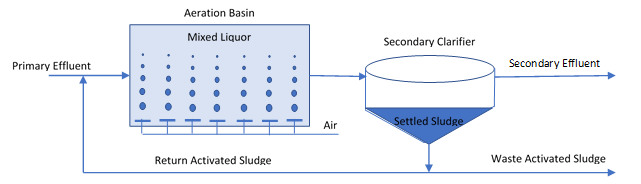
\includegraphics[height=4.5cm]{ASProcess}
\end{center}
\begin{itemize}

\item Utilizes an aeration basin/reactor and a secondary clarifier

\item In the presence of oxygen, aerobic bacteria in the aeration basin consume the organic matter (BOD) in wastewater for their growth and reproduction, converting BOD into bacterial cell mass along with metabolic byproducts including carbon dioxide and water

\item The aerobic bacteria is the predominant microbial life form in the aeration basin.  Other higher microbial life forms — mainly protozoa, are present along with some metazoans.

\item The microorganisms along with their metabolic byproducts and residual dead cell mass form a cluster called floc.

\item The wastewater exiting the aeration basin enters a clarifier where the floc settles.  The clear, treated secondary effluent flows out.

\item A portion of the settled activated sludge floc, is returned from the clarifier to the front of the aeration basin to seed the activated sludge treatment of the incoming primary effluent. The recycled floc is called \textbf{Return Activated Sludge (RAS)}.

\item The remaining settled floc from the clarifier is ”wasted” \textemdash transferred for solids treatment (typically using digestion) prior to its ultimate disposal. The wasted floc is called \textbf{Waste Activated Sludge (WAS)}.

\item The color of healthy activated sludge is tan to brown with an earthy/musty odor.

\item For activated sludge treatment to be effective, it is critical to establish a healthy microbial population which \hl{converts the BOD} into \hl{easily separable biomass.}
\item If the biomass does not settle well in the clarifier, it will be carried out in the treated secondary effluent producing a poor quality effluent with higher solids and organic content.  \\
\end{itemize}


\subsection{Pond System}\index{Pond System}
Similar to the suspended growth, stabilization ponds are large man made bodies of water which treat wastewater using mainly natural processes including sunlight, algae and microorganisms.
\begin{itemize}
\item Stabilization ponds and lagoons are bodies of water which treat wastewater using mainly natural processes including sunlight, algae and microorganisms for treating wastewater\\
\item While ponds are shallow and man-made, lagoons are bodies of water confined within natural boundaries.\\
\end{itemize}

 , which break down the effluent. It is in the anaerobic pond that the influent begins breaking down in the absence of oxygen "anaerobically". The anaerobic pond acts like an uncovered septic tank. Anaerobic bacteria break down the 

\subsubsection{Anaerobic Ponds}\index{Anaerobic Ponds}	

\begin{itemize}	
\item Typically for treating raw sewage
\item These are deep - 10-14 feet treatment ponds which rely primarily on anaerobic bacteria to break down the organic waste.
\item Designed for BOD removal
\item High strength wastewater may be treated.
\item Organic matter is broken down releasing releasing methane, carbon dioxide and odorous gases including hydrogen sulfide. 
\item Most of the decomposition is accomplished by acid forming bacteria. 
\item The pH in these lagoons is usually below 6.5. 
\item They are total retention and do not have an effluent discharge. 
\item The anaerobic pond must be de-sludged approximately once every 2 to 5 years
\item Organic loading of 200-1000 lbs. $BOD_5$ per acre per day
\end{itemize}

\subsubsection{Facultative Ponds}\index{Facultative Ponds}	

\begin{itemize}
\item The depth of facultative ponds is about 4-7 feet which is in-between the depths of anaerobic ponds (10-14 feet) and aerobic ponds 3 feet)
\item The uper layer of facultative pond is aerobic, and bottom layer is mostly anaerobic.
\item Facultative bacteria are responsible for most of the treatment that occurs in these ponds.  Facultative bacteria are bacteria which can live under both aerobic and anaerobic conditions.
\item The algae that grow in the pond are critical to the successful stabilization of the organic load. 
\item The algae will take in carbon dioxide ($CO_2$) and, through photosynthesis, use it to create sugars and release dissolved oxygen ($O_2$) that is used by the aerobic bacteria. Facultative lagoon levels should always maintain at least 4 feet of water in the pond.
\item Typically for secondary treatment - BOD removal
\item 15-50 lbs $BOD_5$ per acre per day.
\item Unused CO$_2$ will react with water to form carbonic acid - which would reduce the pH unless consumed
\item Sludge removal need is rare.  Sludge can be removed by using a raft-mounted sludge pump or by draining and dewatering the pond and removing the sludge with a front-end loader.
\end{itemize} 

				\begin{sidewaysfigure}
\begin{center}
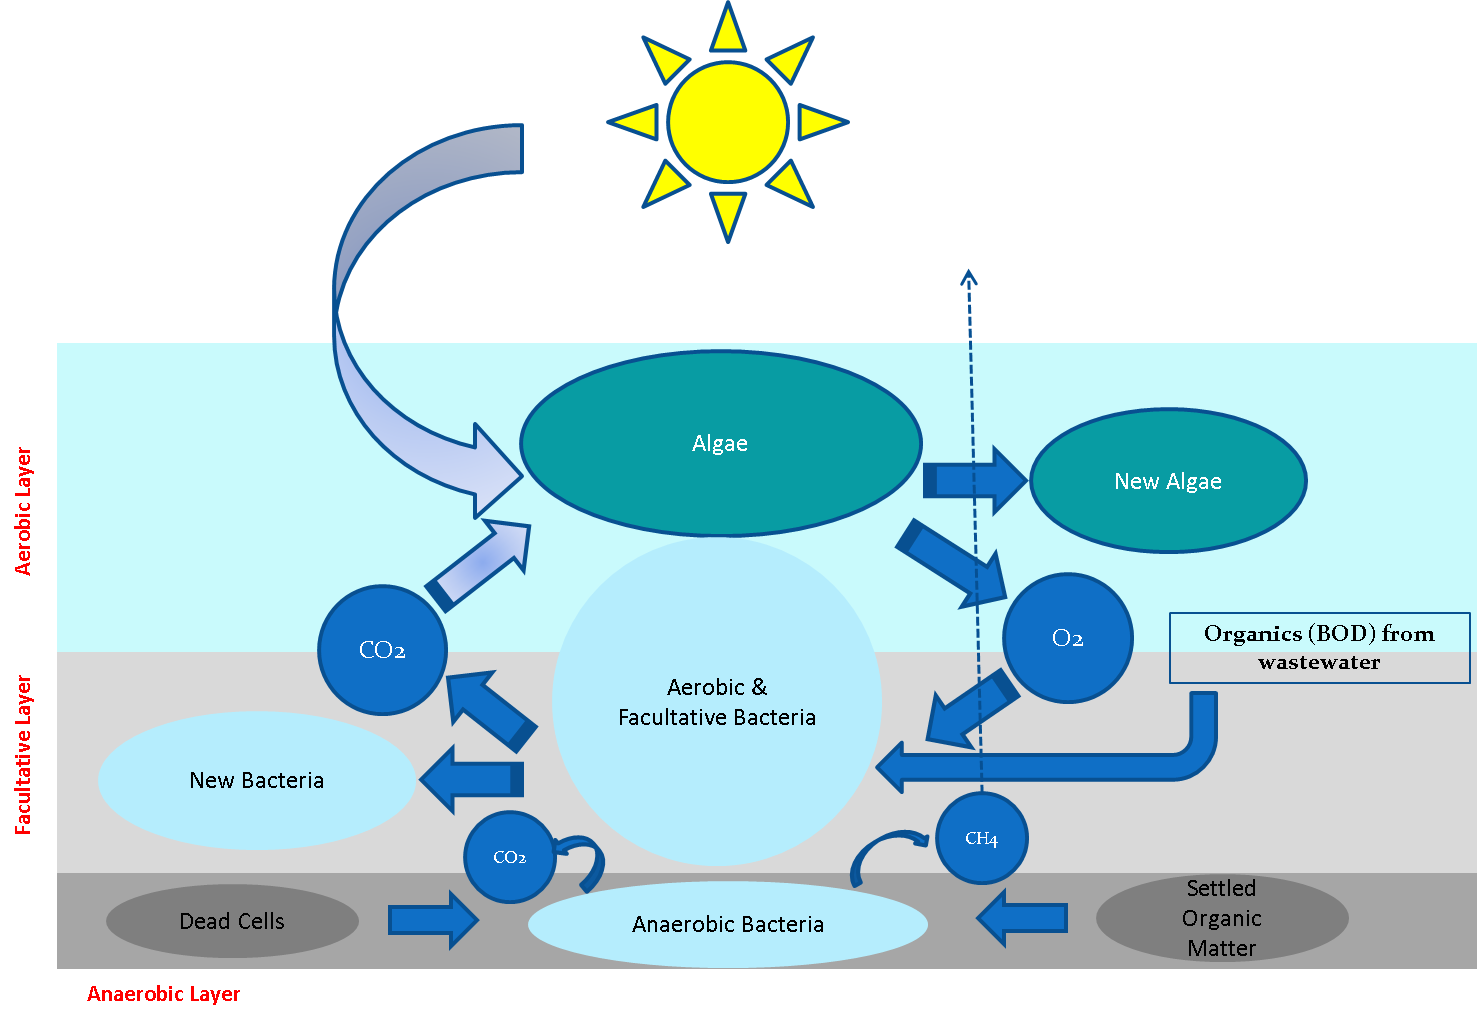
\includegraphics[scale=0.8]{StabilizationPond}\\
Facultative pond schematic
\end{center}
				\end{sidewaysfigure}
				
\subsubsection{Aerobic Stabilization Ponds}\index{Aerobic Stabilization Ponds}
	
Aerobic stabilization ponds are also known as: \hl{maturation}, \hl{polishing} or \hl{finishing} Pond
\begin{itemize}
\item Contain disssolved oxygen throughout entire depth of the pond.
\item Treatment is accomplished through the stabilization of organic wastes by aerobic bacteria and algae.
\item Typically for tertiary treatment
\item Designed for pathogen removal
\item Shallow - only about 3 feet deep. 
\item They are most often the final cells in a multi-staged pond system
\item They are also used as polishing ponds for tertiary treatment of trickling filter plant effluent.
\item Usually the effluent is directed into a second pond where the sludge can settle 
\item Their shallow depth allows sunlight to penetrate to the bottom of the pond to encourage algae growth and aerobic conditions throughout the pond 
\item The low solids loading found in these tertiary treatment applications means that these ponds normally have no sludge zone
\item These ponds may be mechanically aerated 
\item Aerobic polishing ponds are designed for 15-20 pounds BOD/acre/day
\item Aerobic ponds are typically designed for pathogen removal
\item Aerobic lagoon levels should always maintain at least 18 inches of water in the pond
\end{itemize}



